\section{Switch and Diode voltage drop limitations}\label{ch:DROPS}

All the calculation in the report until this point were done assuming all components were ideal. Since it was concluded the 2Nx Multilevel BC is the topology that will be build in hardware, we will need to calculate the expected drops as well, to see if the real results are close to the simulations we have ran. 
The same structure will be followed as the previous section, where a 3x non-inverting BC will be analysed and the calculations will be mirrored to achieve the 2Nx combination.

The components considered significant are diodes and switches.Other research papers (\cite{Padmanaban2015,Rosas-Caro2008}) assume the drops across the two are equal. Our goal is two separate the two to improve the accuracy of the model. Since the voltage drop is constant and can be measured (usually also denoted in specification sheets), the rest of the losses can be accounted to the switch.

\subsubsection{3x Non-inverting}

First, the relationship between the components will be derived afterwards we will be able to link it to the input output relationship.

\begin{figure}[H]%
    \centering
    \subfloat[Loop 1]
    {{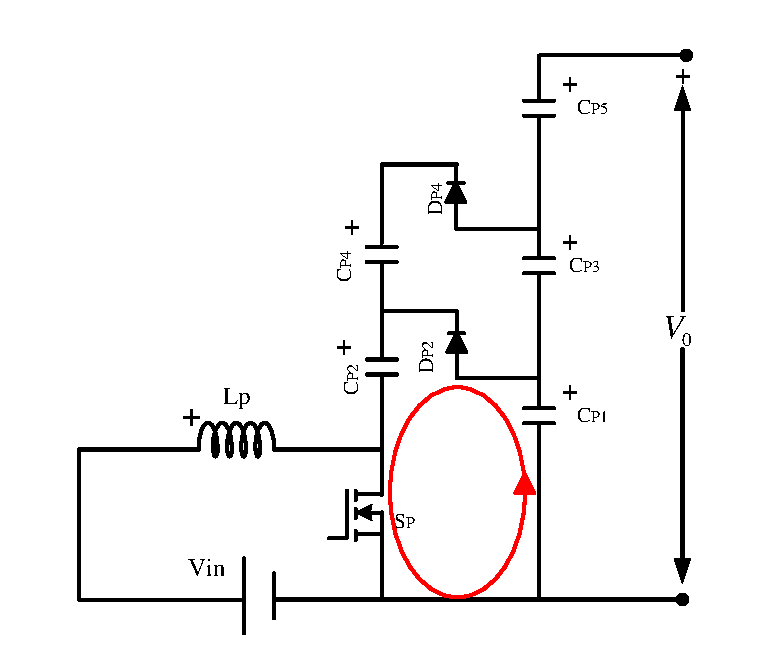
\includegraphics[width=0.4\textwidth]{figures/zComponentDrops/DROPS_LOOP1.pdf} \label{fig:DROPS_LOOP1}}}%
    \qquad
    \subfloat[Loop 2]{{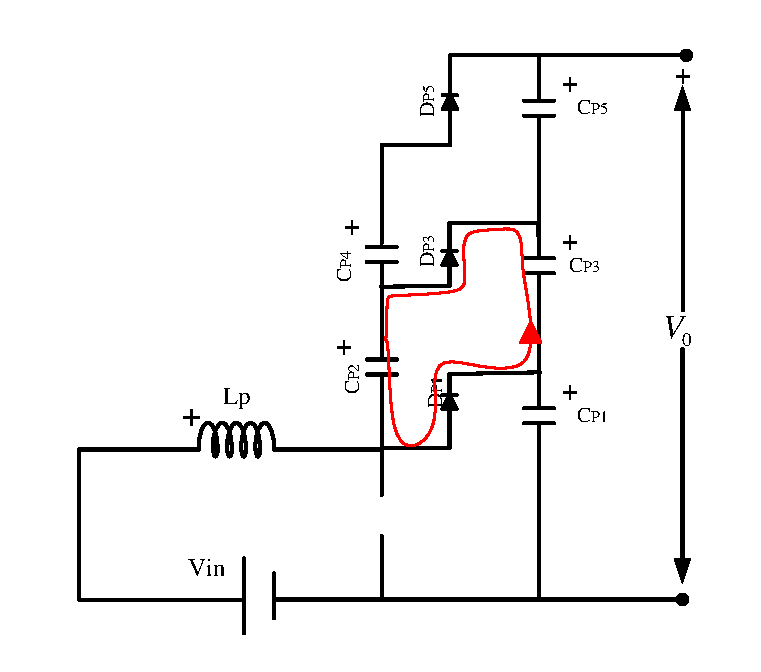
\includegraphics[width=0.4\textwidth]{figures/zComponentDrops/DROPS_LOOP2.pdf} \label{fig:DROPS_LOOP2}}}%  
   \qquad
        \subfloat[Loop 3]
    {{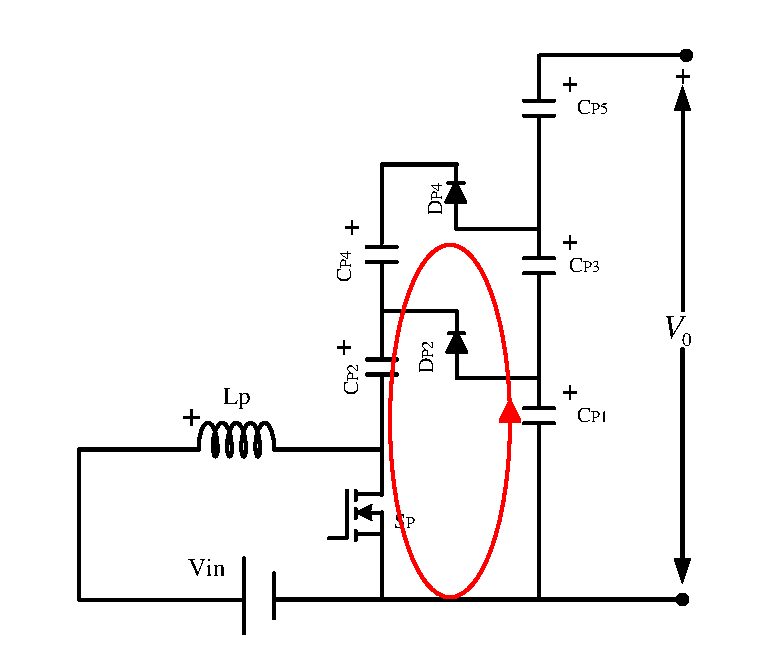
\includegraphics[width=0.4\textwidth]{figures/zComponentDrops/DROPS_LOOP3.pdf} \label{fig:DROPS_LOOP3}}}%
    \qquad
    \subfloat[Loop 4]{{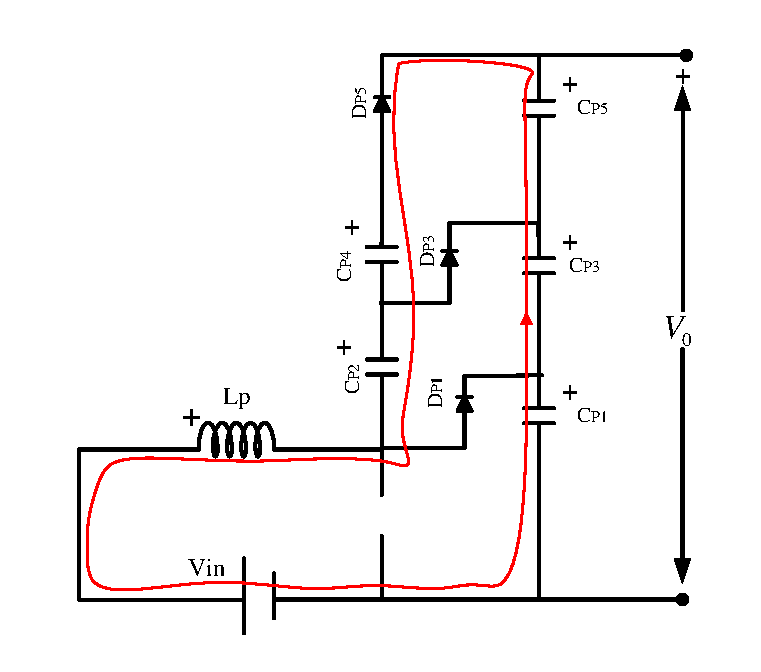
\includegraphics[width=0.4\textwidth]{figures/zComponentDrops/DROPS_LOOP4.pdf} \label{fig:DROPS_LOOP4}}}%  
    \caption{Loops required to calculate the voltage drops}%
     \label{fig:DROPS_LOOPS}% 
     
\end{figure}

Starting with the loop marked of Fig. \ref{fig:DROPS_LOOP1}, we follow the lines and every time one of the components we considered significant is passed through, the expected voltage drop ($V_D$ or $V_{Sw}$) is subtracted.

So the KVL equation is as follows: 
\begin{equation}
	V_{Cp2} = V_{Cp1}-V_{Sw}-V_D
	\label{eq:LOOP1}
\end{equation}

Now the switch is turned off and the loop marked on Fig. \ref{fig:DROPS_LOOP2} can be expressed via KVL: 
\begin{equation}
	V_{Cp3} = V_{Cp2}=V_{Cp1}-V_D-V_{Sw}
	\label{eq:LOOP2}
\end{equation}
After another turn of the switch we can build the expression for the loop marked on figure Fig. \ref{fig:DROPS_LOOP3}:
\begin{equation}
	V_{Cp3}+V_{Cp1}-V_{Sw}-V_{Cp2}-V_{Cp4}-V_D=0
	\label{eq:LOOP3_1}
\end{equation}
With the help of Eq. \ref{eq:LOOP1} the term is reduced to:
\begin{equation}
	V_{Cp3} = V_{Cp4}
	\label{eq:LOOP3_2}
\end{equation}
Lastly, in the loop of Fig. \ref{fig:DROPS_LOOP4} with the switch in OFF state:
\begin{equation}
	V_L-V_{Cp2}-V_{Cp4}-V_D+V_{Cp5}+V_{Cp3}+V_{Cp1}-V_{in}= 0
	\label{eq:LOOP4_1}
\end{equation}
On the same figure, a loop identical to the CBC OFF state can be formed as well making:
\begin{equation}
	V_{Cp1}=V_{in}+V_L-V_D
	\label{eq:LOOP4_2}
\end{equation}
In Eq. \ref{eq:LOOP3_2} it was already concluded $V_{Cp3}$ and $V_{Cp4}$ are equal. Consequently: 
\begin{equation}
	V_{Cp2} = V_{Cp5}
	\label{eq:LOOP4_3}
\end{equation}
Referring back to Eq. \ref{eq:LOOP1} and Eq. \ref{eq:LOOP2}: 
$V_{Cp4}$ are equal. Consequently: 
\begin{equation}
	V_{Cp5}=V_{Cp1}-V_D-V_{Sw} =V_{Cp3} 
	\label{eq:LOOP4_4}
\end{equation}
If we extend this circuit to the general Nx non-inverting BC,voltages over the capacitors after $C_{p1}$ on the output side will be equal to the term calculated for $V_{Cp3}$ and  $V_{Cp5}$. Generalised we can express the voltage across the $C_{p(2N-1)}$ capacitor as: 
\begin{equation}
	V_{Cp(2N-1)}= V_{Cp1}-V_D-V_{Sw} 
	\label{eq:C_2N-1}
\end{equation}

As already proven in Section \ref{ch:MBC} the output voltage can be generalised as the sum of the voltages across all the output side capacitors: 
\begin{equation}
	V_{Top}= NV_{Cp1}-(N-1)V_D-(N-1)V_{Sw} 
	\label{eq:DROPS_V_TOP}
\end{equation}
Now all all we need to define is as expression for $V_{Cp1}$ including the voltage drops. To do achieve that, we look back to Figure. \ref{fig:MBC_3XFULL}. The first level of the circuit is basically a conventional boost converter, therefore we will looked deeper into how the diode and switch influence the output of a conventional BC. 
\vspace{2mm}
\subsubsection{Conventional boost converter}

To avoid doing the whole deriviation a second time, referring back to Eq. \ref{eq:CBC_SWON1} and Eq. \ref{eq:CBC_SWOFF1} and add the switch and diode drop respectively. Consequently combining the two using the IVSB, we easily get an expression for the output voltage \cite{BoostSwi93:online}
\vspace{2mm}
\begin{equation}
	V_{O}= \frac{V_{in}-V_{Sw}D}{1-D}-V_D
	\label{eq:DROPS_CONV}
\end{equation}

The output voltage of a conventional BC can be substitute with the voltage across the first capacitor in the Nx Multilevel BC, this turns Eq. \ref{eq:DROPS_V_TOP} into: 
\vspace{2mm}
\begin{equation}
	V_{O}= N( \frac{V_{in}-V_{Sw}D}{1-D}-V_D)-(N-1)V_D-(N-1)V_{Sw} 
	\label{eq:DROPS_NX_FINAL}
\end{equation}

Finally, we need to get back to the initial goal and calculate the formula for the output of a 2Nx multilevel BC. 
In contrast to Sec. REFER TO 2NX the inverting part of the full topology isn't just a mirror version of the non-inverting. The main difference is that the conventional BC gain falls on Cp' from Fig. \ref{fig:MBC_2NxSchematic}. Therefore one more pair of drops will occur on the output side, as all the voltages across all capacitors apart from the initial ones are equal. In conclusion the output voltage on the bottom side of the converter is:
\begin{equation}
	V_{Bot}= N(\frac{V_{in}-V_{Sw}D}{1-D}-V_D)-NV_D-NV_{Sw} 
	\label{eq:DROPS_V_BOT}
\end{equation}

Consequently, combining the two halves of the converter: 
\begin{equation}
	V_{O}=V_{Top}+V_{Bot}=2N( \frac{V_{in}-V_{Sw}D}{1-D}-V_D)-(2N-1)V_D-(2N-1)V_{Sw}
	\label{eq:DROPS_2INX_FINAL}
\end{equation}

\subsubsection{Simulation}

In order to verify that the calculated drops are correct,
the topology was built in LTSpice this time. 
Again, the same parameters for the components were used as the other topologies as observed on Table~\ref{tab:MBC_2Nx}. 
For the switch and diode models were taken from the producers databases. 
The exact MOSFET and diode are discussed further in the next sections, while their drops were approximated form the simulations.
The full simulation circuit is included in the Appendix. 

\begin{table}[H]
\begin{center}
\caption {Simulation parameters for MBC} \label{tab:MBC_2Nx} 
\begin{tabular}{|l|l|}
\cline{1-2}
\textbf{Parameter} & \textbf{Value}  \\ \cline{1-2}
Input Voltage $V_{in}$          &      10V   \\ \cline{1-2}
Load(R)   & 225$\Omega$           \\ \cline{1-2}
Capacitance(C)          &       220$\mu$F     \\ \cline{1-2}
Inductance(L)          &      150$\mu$H      \\ \cline{1-2}
Duty cycle(D)          &     0.6       \\ \cline{1-2}
Switching Frequency(f)          &      50kHz      \\ \cline{1-2}
Diode drop ($V_D$)          &     1V       \\ \cline{1-2}
MOSFET drop ($V_{Sw}$)          &     0.6V       \\ \cline{1-2}
\end{tabular}
\end{center}
\end{table}

The expected results with the given value are: 
\begin{equation}
	V_{Top}= N( \frac{V_{in}-V_{Sw}D}{1-D}-V_D)-(N-1)V_D-(N-1)V_{Sw}= 66.1V
	\label{eq:DROPS_NX_SIM}
\end{equation}

\begin{equation}
	V_{Bot}= N(\frac{V_{in}-V_{Sw}D}{1-D}-V_D)-NV_D-NV_{Sw}= 64,5V
	\label{eq:DROPS_V_BOT_SIM}
\end{equation}

\begin{equation}
	V_{O}=2N(\frac{V_{in}-V_{Sw}D}{1-D}-V_D)-(2N-1)V_D-(2N-1)V_{Sw}= 134.2V
	\label{eq:DROPS_2INX_FINAL_SIM}
\end{equation}


The simulated wave forms can be seen on Fig \ref{fig:MBC_2NxSimResult_DROPS}. The results are off from the calculated ones, as the component models introduce some non linearities that involve temperature, which is not part of the scope. However, the relative error is less than 1\% on all values. 

\begin{figure}[H]
   \centering
   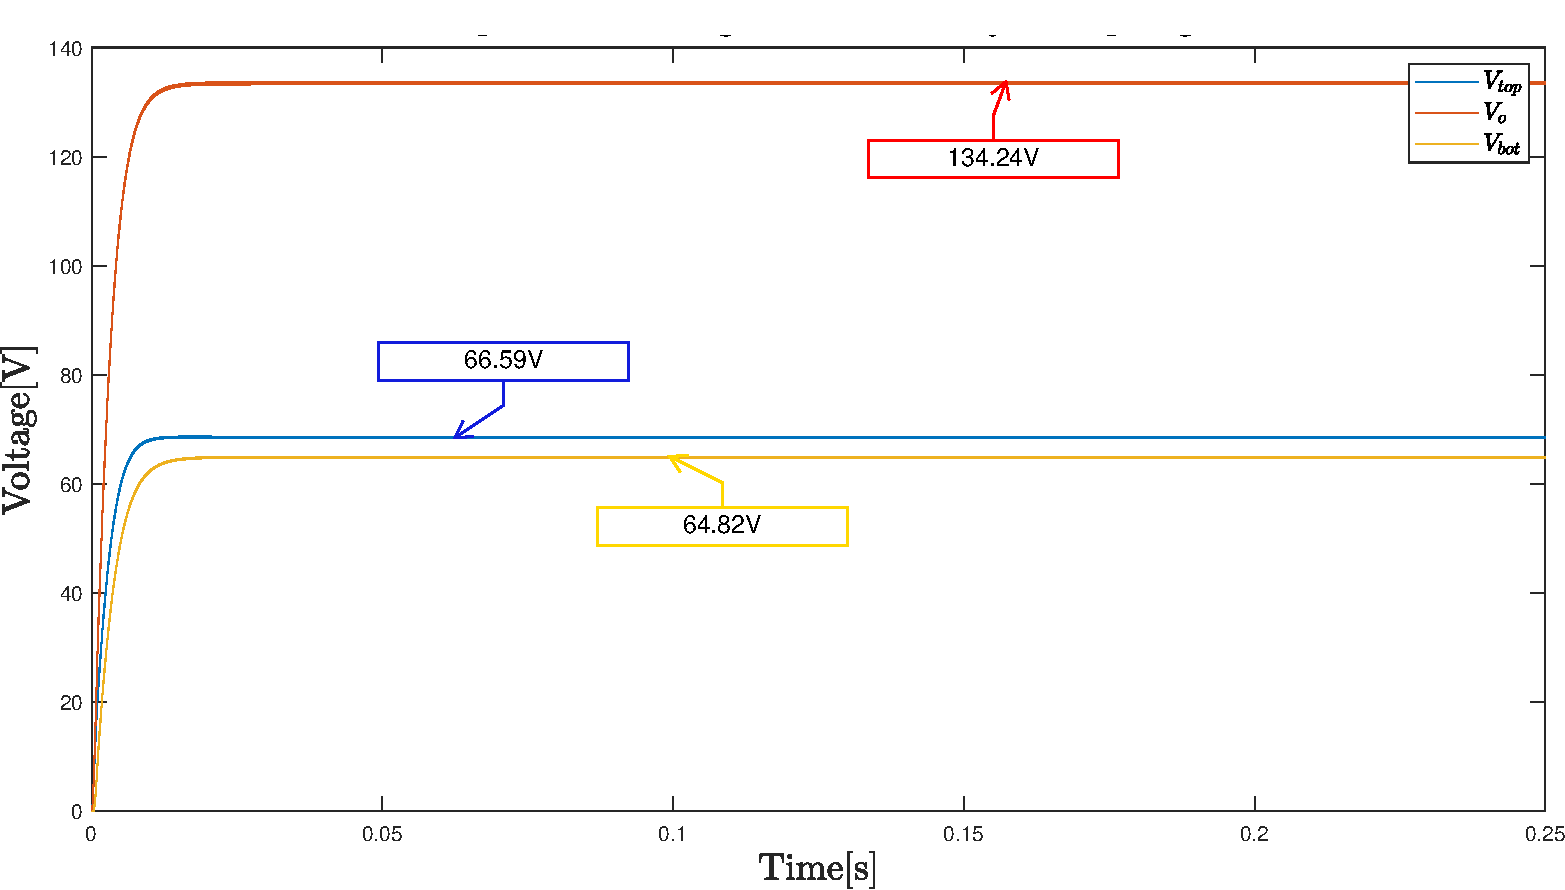
\includegraphics[width=0.8\textwidth]{figures/zComponentDrops/compare_LTSpice.pdf}
    \caption{6x Interleaved BC Simulations results with included components}
	\label{fig:MBC_2NxSimResult_DROPS}
\end{figure}

